\section{Text Management}
\label{sec:textmanagement}
The art and challenge of modularization lie in finding an effective decomposition of a topic into
modules with relatively thin interfaces or, in other words, into modules with a great potential for
information hiding. Text systems provide a welcome opportunity of an exercise. A closer analysis
immediately leads to the following separate concerns corresponding to the components Model,
View and Controller of the MVC scheme: Text management, text rendering, and text editing. If we
combine View and Controller and add an auxiliary font handling module Fonts, we arrive at the
following three-module import hierarchy:
\begin{table}[h!]
  \begin{tabular}{l l l}
    Module     &Object type &Service \\\hline
    TextFrames &Frame       &Text rendering and editing\\
    Texts      &Text        &Text management \\
    Fonts      &Font        &Font management
  \end{tabular}
\end{table}

Note that, in contrast to the display-subsystem, the associated object types are not connected hierarchically here.

Separate Sections 5.3 and 5.4 will be devoted to modules TextFrames and Fonts respectively. In
the current Section we focus on module Texts. Regarding it as a model of the abstract data type
Text presented in the previous Section, its definition is congruent with the specification of the
abstract data type itself, and we need not repeat it here.

The main topics of this Section are internal representation and file representation of texts. We first
emphasize that the internal representation of a text is a completely private matter of module Texts
that is encapsulated and hidden from clients. In particular, the representation could be changed at
any time without invalidating any single client. In principle, the same is true for the file
representation. However, stability is of paramount importance here because files serve the
additional purposes of backing up text on external media and of porting text to other environments.
Our choice of an internal representation of text was determined by a catalogue of requirements and
desired properties. The wish list looks like this:
\begin{enumerate}
  \item lean data structure
  \item closed under editing operations
  \item efficient editing operations
  \item efficient sequential reading
  \item efficient direct positioning
  \item super efficient internalizing
  \item preserving file representations
\end{enumerate}
With the exception of 5, we found these requirements met perfectly by an adequately generalized
variant of the piece list technique that was originally used for Xerox PARC's Bravo text editor and
also for ETH's former document editors Dyna and Lara [Gutknecht]. The original piece list is able to
describe a vanilla text without looks. It is based on:
\begin{itemize}
  \item A text is regarded as a sequence of pieces, where a piece is a section of a text file
    consisting of a sequence of contiguous characters.
  \item Each piece is represented by a descriptor \verb|(f, pos, len)|,
    designating $file$, starting $position$, and $length$ respectively.
    The whole text is represented as a list of piece descriptors (in short: \emph{piece list}).
    The editing operations operate on the list rather than on pieces themselves.
\end{itemize}

\begin{figure}[h!]
  \centering
  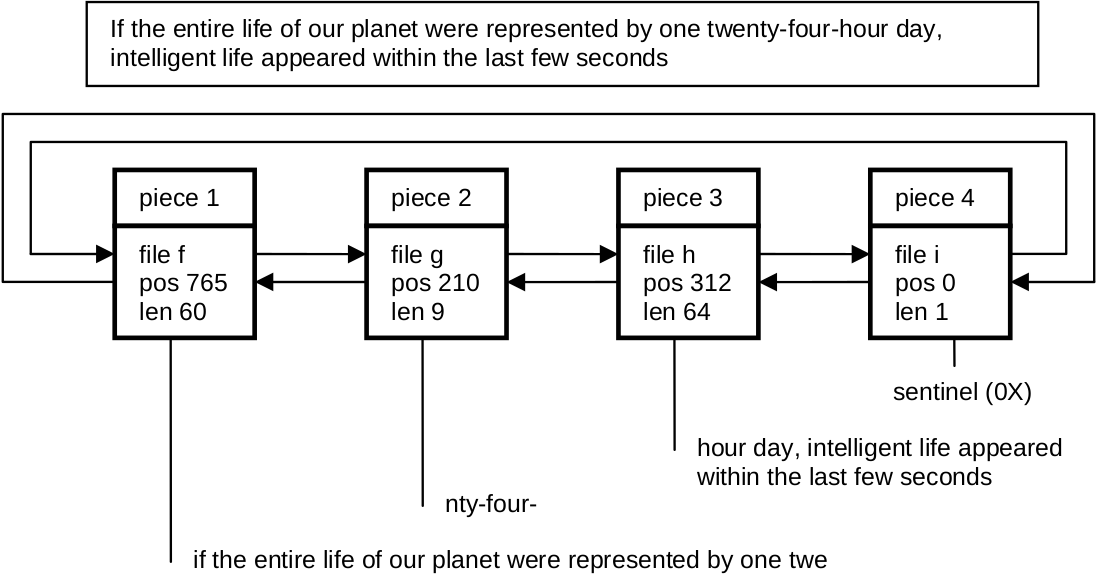
\includegraphics[width=.8\textwidth]{i/d}
  \caption{Piece chain representing a text}
  \label{fig:chain}
\end{figure}
Fig \ref{fig:chain} shows a typical piece list representing (the current state of) a text.
Investigating the effects of the basic editing operations \emph{delete} and \emph{insert}
on this piece list, we end up with these algorithms:
\begin{verbatim}
delete stretch [beg, end) of text = BEGIN
  split pieces at both beg and end;
  remove p-descriptors from beg to end from the chain
END

insert stretch of text at pos = BEGIN
  split piece at pos;
  insert p-descriptors representing the stretch there
END
\end{verbatim}
Splitting is superfluous if the desired splitting point happens to coincide with
the piece beginning.  Fig \ref{fig:chain-after-insert} and \ref{fig:chain-generalized}
show the resulting list after a delete, and an insert respectively:
\begin{figure}[h!]
  \centering
  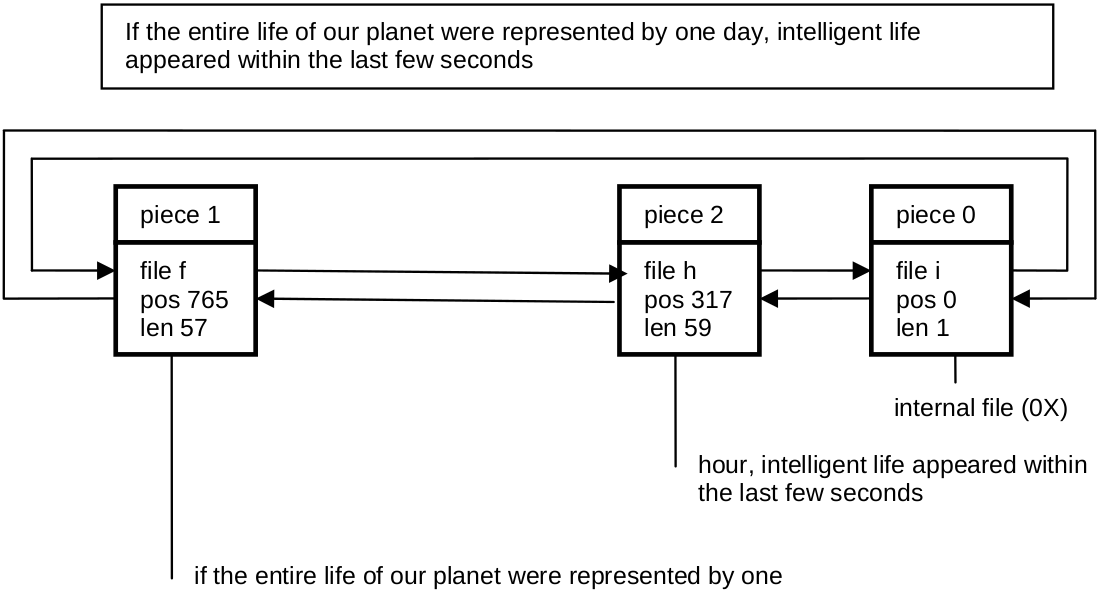
\includegraphics[width=.8\textwidth]{i/e}
  \caption{Piece chain after delete operation}
  \label{fig:chain-after-delete}
\end{figure}
\begin{figure}[h!]
  \centering
  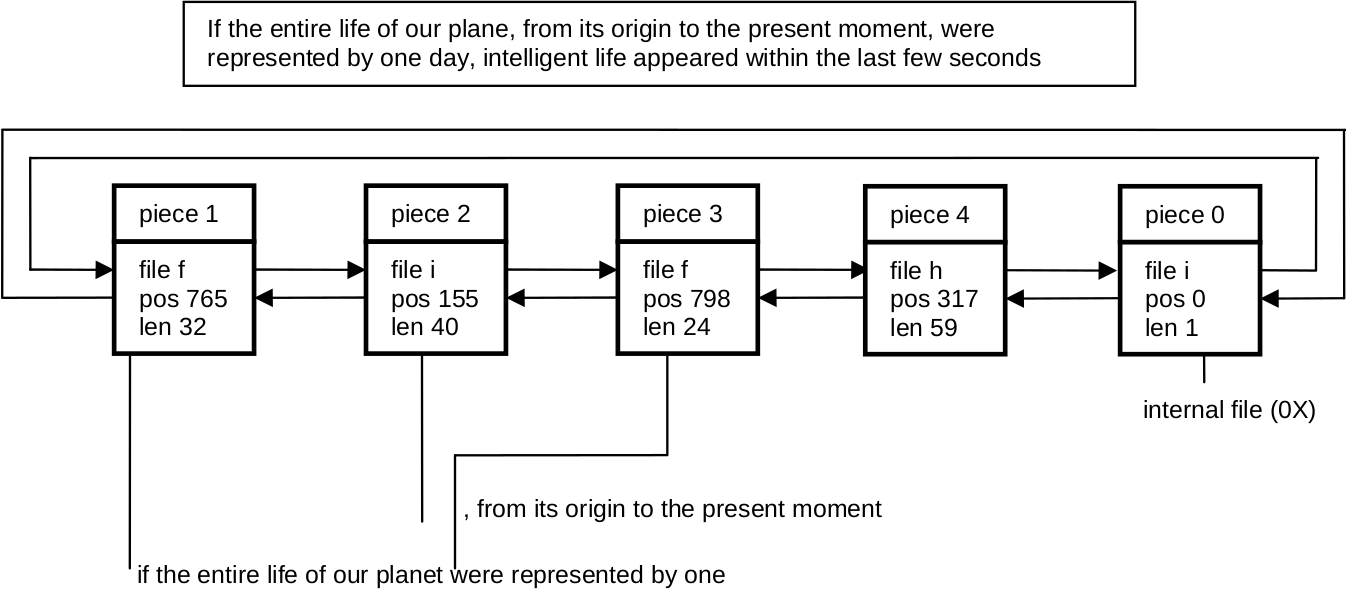
\includegraphics[width=.8\textwidth]{i/f}
  \caption{Piece chain after insert operation}
  \label{fig:chain-after-insert}
\end{figure}

Checking our above wish list we immediately recognize the requirements 1, 2, and 3 as met.
Requirement 4 is also met assuming an efficient mechanism for direct positioning in files.
Requirement 6 can be checked off because the piece list initially consists of a single piece
spanning the entire text file.  Finally, requirement 7 is met simply because the operations
do not affect file representations at all.

In Oberon we adapted the piece list technique to texts with looks (\emph{rich texts}).
Formally, we 1st define a run as a stretch of text whose characters show identical looks.
Now, we require the piece list to subordinate itself to the run structure.
This obviously means that every piece needs to be contained within a single run.
Fig \ref{fig:chain-generalized} visualizes such a compliant piece list representing a text
with varying looks.  There are only 2 new aspects compared to the original version
of the piece list discussed above:
An additional operation to change looks and the initial state of the piece chain.
\begin{verbatim}
change looks in a stretch [beg, end) of text = BEGIN
  split pieces at both beg and end;
  change looks in piece descriptors from beg to end
END
\end{verbatim}
This shows that wish list requirements 2 and 3 still satisfied.
\begin{figure}[h!]
  \centering
  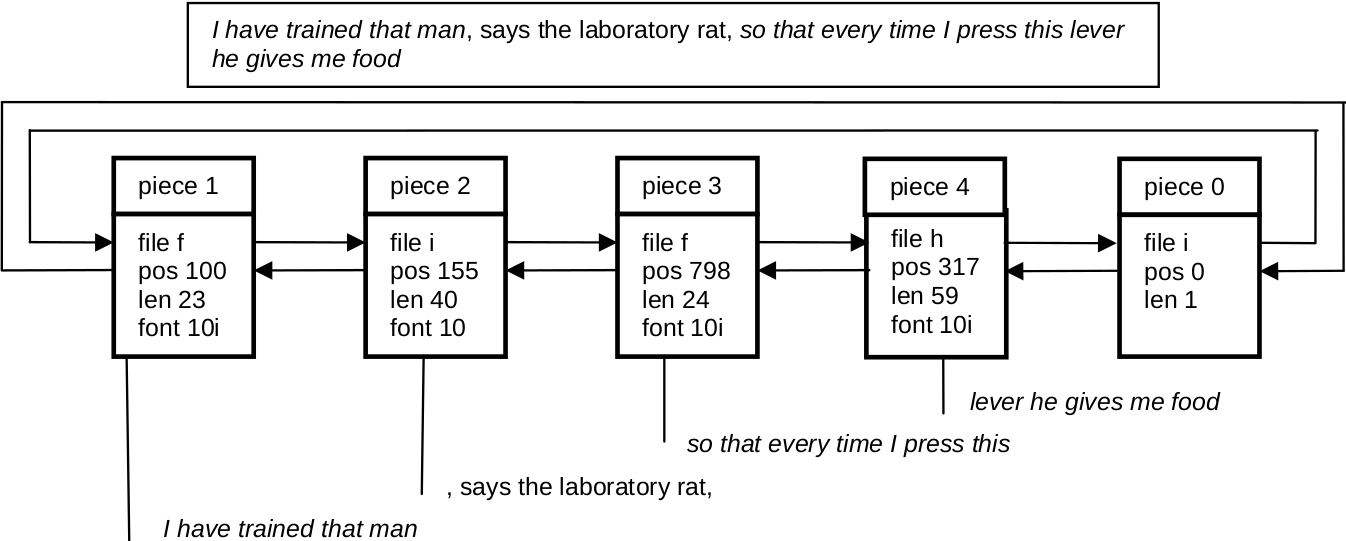
\includegraphics[width=.8\textwidth]{i/g}
  \caption{Generalized piece chain representing a rich text}
  \label{fig:chain-generalized}
\end{figure}

Initially, the pieces are identical with runs, and the number of elements in the piece list
is equal to the one of runs.  Because this number is typically small in comparison with
the total characters number in a text, requirement 6 is still met.

We conclude that the new aspects do not invalidate the positive rating given above
to the piece technique with regard to wish list requirements 1-4, 6 and 7.  However,
requirement of efficient direct positioning remains.  The problem is the necessity
to scan through the list sequentially to locate the piece that contains the desired position.
We investigated different solutions of this efficiency problem.  They are based on
different data structures connecting the piece descriptors, among them a piece tree
and a variant of the piece list featuring an additional long-distance link like in a skip-list.

Eventually, we decided in favor of a simpler solution that we can easily justify
by pointing out that the typical editing scenario is zooming into a local region of text,
i.e. positioning at an arbitrary location once and subsequently positioning at locations
in its immediate neighborhood many times.  Therefore, an appropriate solution is
caching the most recently calculated values \verb|(pos, piece)| of the translation map.
Of course, this does not solve the problem of cache misses.  Notice, however, that
this problem is acute only in the case of extremely long piece lists that do not occur
in ordinary texts and editing sessions.

We shall now illustrate the piece technique in detail
at the example of 2 important but basic operations: Insert and read.
Let us start with an overview of the data types involved.
Apart from some auxiliary private variables marked with an arrow,
the types \verb|Text|, \verb|Buffer|, and \verb|Reader| are already familiar to us
from the previous Section.  \verb|Piece| is completely private and hidden from the clients.
\begin{verbatim}
  Text = POINTER TO TextDesc;
  Notifier = PROC(T: Text; op, beg, end: INT);
 
  TextDesc = RECORD len: INT; notify: Notifier;
               --> trailer: Piece;
               --> org: INT;
               --> pce: Piece
             END;
 
  Buffer = POINTER TO BufDesc;
  BufDesc = RECORD len: INT;
              --> header, last: Piece
            END;
  
  Reader = RECORD eot: BOOL; fnt: Fonts.Font;
             col, voff: INT;
             --> ref: Piece;
             --> org, off: INT;
             rider: Files.Rider
           END;
  
  --> Piece = POINTER TO PieceDesc;
  --> PieceDesc = RECORD f: Files.File;
                    off, len: INT;
                    fnt: Fonts.Font;
                    col, voff: INT;
                    prev, next: Piece
                  END;
\end{verbatim}

As depicted in Fig \ref{fig:chain}, the piece list is implemented as a doubly linked list
with a sentinel piece closing it to a ring.
The field trailer in \verb|TextDesc| points to the sentinel piece.
Fields \verb|org| and \verb|pce| implement a translation cache consisting of merely one entry
\verb|(org, pce)|.  It links a position \verb|org| with a piece \verb|pce|.
The fields \verb|header| and \verb|last| in \verb|Buffer| refer to the implementation
of buffers as piece lists.  They point to the first and last piece descriptors respectively.
Finally, the fields \verb|ref|, \verb|org|, and \verb|off| in \verb|Reader|
memorize the current piece, its origin, and the current offset within this piece.
The fields \verb|f|, \verb|off|, and \verb|len| in \verb|Piece| specify the underlying file,
starting position in the file, and length of the piece.
\verb|fnt|, \verb|col|, and \verb|voff| are its looks.
Finally \verb|prev| and \verb|next| are pointers to the previous and next piece in the list respectively.

\verb|FindPiece| and \verb|SplitPiece| are auxiliary procedures
that are used by almost all piece-oriented operations.
\begin{verbatim}
 PROC FindPiece(T: Text; pos: INT; VAR org: INT; VAR p: Piece);
   VAR p: Piece; porg: INT;
 BEGIN p := T.pce; porg := T.org;
1) IF pos >= porg THEN
     WHILE pos >= porg + p.len DO INC(porg, p.len); p := p.next END
2) ELSE p := p.prev; DEC(porg, p.len);
     WHILE p < porg DO p := p.prev; DEC(porg, p.len) END
   END;
3) T.pce := p; R.org := porg; (*update cache*)
   pce := p; org := porg
 END FindPiece;
\end{verbatim}

Explanations (referring to the line numbers in the above code excerpt)
1) search to the right (next)
2) search to the left (prev)
3) update cache if more than 50 pieces traversed

\begin{verbatim}
1) PROC SplitPiece (p: Piece; off: INT; VAR pr: Piece);
     VAR q: Piece;
   BEGIN
2)   IF off > 0 THEN NEW(q);
       q.fnt := p.fnt; q.col := p.col; q.voff := p.voff;
       q.len := p.len - off;
       q.f := p.f; q.off := p.off + off;
       p.len := off;
3)     q.next := p.next; p.next := q;
4)     q.prev := p; q.next.prev := q;
       pr := q
     ELSE pr := p
     END
   END SplitPiece;
\end{verbatim}

Explanations:
1) return right part piece pr after split
2) generate new piece only if remaining length > 0
3) insert new piece in forward chain
4) insert new piece in backward chain

Procedure Insert handles text insertion. It operates on a buffer that contains the stretch of text to be inserted:
\begin{verbatim}
 PROC Insert (T: Text; pos: INT; B: Buffer);
   VAR pl, pr, p, qb, qe: Piece; org, end: INT;
 BEGIN
1) FindPiece(T, pos, org, p); SplitPiece(p, pos - org, pr);
2) IF T.org >= org THEN
     T.org := org - p.prev.len; T.pce := p.prev
   END;
   pl := pr.prev; qb := B.header.next;
3) IF (qb # NIL) & (qb.f = pl.f) & (qb.off = pl.off + pl.len)
    & (qb.fnt = pl.fnt) & (qb.col = pl.col) & (qb.voff = pl.voff) THEN
     pl.len := pl.len + qb.len; qb := qb.next
   END;
   IF qb # NIL THEN qe := B.last;
4)   qb.prev := pl; pl.next := qb; qe.next := pr; pr.prev := qe
   END;
5) T.len := T.len + B.len; end := pos + B.len;
6) B.last := B.header; B.last.next := NIL; B.len := 0;
7) T.notify(T, insert, pos, end)
 END Insert;
\end{verbatim}

Explanations:
1) split piece to isolate point of insertion
2) adjust cache if necessary
3) merge pieces if possible
4) insert buffer
5) update text length
6) empty buffer
7) notify

Procedure Read implements sequential reading of characters in texts. It operates on a text reader:
\begin{verbatim}
 PROC Read (VAR R: Reader; VAR ch: CHAR);
 BEGIN
1) Files.Read(R.rider, ch); R.fnt := R.ref.fnt; R.col := R.ref.col; R.voff := R.ref.voff;
   INC(R.off);
2) IF R.off = R.ref.len THEN
3)   IF R.ref.f = WFile THEN R.eot := TRUE END;
     R.org := R.org + R.off; R.off := 0;
4)   R.ref := R.ref.next; R.org := R.org + R.off; R.off := 0;
5)   Files.Set(R.rider, R.ref.f, R.ref.off)
   END
 END Read;
\end{verbatim}

Explanations:
1) read character from file and update looks in reader
2) if piece boundary reached
3) check if sentinel piece reached
4) move reader to next piece
5) position file rider

Procedure Read is typically used as a primitive by text scanners and in particular by the built-in
scanner Scan for the recognition of universal tokens, as they were defined in the previous section.
Scanning is a rather complex operation that, for example, includes the conversion of a sequence of
digits into an internal floating-point representation and vice-versa. Scanning a real number involves
recognizing m and d, and computing x = m*10d. This is done using procedure Ten(d) computing 10d
by repeated multiplication maintaining the invariant t * pn = 10n0, where n0 is the initial value of n.
\begin{verbatim}
  PROC Ten(n: INT): REAL;
    VAR t, p: REAL;
  BEGIN t := 1.0; p := 10.0;
    WHILE n > 0 DO
    IF ODD(n) THEN t := p * t END ;
    p := p*p; n := n DIV 2
    END ;
    RETURN t
  END Ten;
\end{verbatim}

Writing a real number in decimal form is more complicated. It involves the computation of m and d
from x = n*2e so that x = m*10d with \verb|1.0 \leq m < 10.0|. First, e is obtained with the standard function
UNPK(x, e), then d is computed (from the relationship 10k = 2k*log(10)) as d = e/log2(10). In order to
avoid a real division for obtaining d, we use the approximation 1.0 / log2(10) = 77 DIV 256, and then
compute x := x / Ten(e) or x := x * Ten(-e). Further details are to be taken from the listings of
WriteReal and WriteRealFix.

In spite of its apparent simplicity the piece list technique interoperates with other system
components in quite a subtle way. For example, after a while of editing, there are typically
numerous cross references between the documents involved. In other words, pieces of one
document may point to foreign files that is to files that were originally associated with other
documents. As a consequence, the FS must either employ some smart garbage collection
algorithm or not recycle file pages at all, even if a new version of a file of the same name has been
created in the meantime.

A problem of another kind, again affecting the FS, arises if, say, a single text line is
composed of several small pieces. Then, reading this line sequentially may necessitate several
jumps to different positions in different files at a high pace. Depending on the quality of the file
buffering mechanism, this may lead to significantly hesitant mouse tracking.

And finally, typed characters that are supposed to be inserted into a text need to be stored on the
so-called keyboard file. For this (continuously growing) file, several readers and one writer must be
allowed to coexist concurrently.

As a consequence, the following qualities of the underlying FS are mandatory for the piece technique to work properly:
\begin{enumerate}
  \item Once a file page is allocated it must not be reused (until system restart).
  \item A versatile file buffering mechanism supporting multiple buffers per file is required.
  \item Files must be allowed to be open in read mode and in write mode simultaneously.
\end{enumerate}
The format of text sections in files obeys a set of syntactical rules (productions) that can easily be
specified in EBNF-notation:
\begin{verbatim}
  TextSection = ident header {char}.
  header = type offset run {run} null length.
  run = font [name] color offset length.
\end{verbatim}

In the \verb|TextSection| production \verb|ident| is an identifier for text blocks. In the \verb|header| production
\verb|type| is a type-discriminator, \verb|offset| is the offset to the character part, \verb|run| is a run-descriptor,
\verb|null| is a nullcharacter, and \verb|length| is the length of the character sequence. In the \verb|run| production
\verb|font|, \verb|color|, and \verb|offset| are specifications of looks, and \verb|length| is the run-length.
In order to save space, font names are coded as ordinal numbers within a text section. If and only if a font appears
for the first time in a text block it is followed by the actual font name.

Let us conclude this Section with 2 side-remarks and a summary.
\begin{itemize}
  \item Remarks:
\begin{enumerate}
  \item For compatibility reasons, plain ASCII-files are accepted as text files as well. They are mapped
    to texts consisting of a single run with standard looks.
  \item Internalizing a text section from a file is extremely efficient because it is obviously sufficient to
    read the header and translate it into the initial state of the piece list.
\end{enumerate}

  \item Summary:\\
    The mechanism used for the implementation of the abstract data type \verb|Text| is completely hidden
    from clients. It is a generalized version of the original piece list technique, adapted to texts with
    looks. The piece list technique in turn is based on the principle of indirection: Operations operate
    on descriptors of texts rather than on texts themselves. The benefits are efficiency and non-destructive
    operations. However, the technique works properly only in combination with an efficient (and reliable)
    garbage collector and a suitable FS.
\end{itemize}
